\documentclass[man,bazy,a4paper,11pt,sfheadings,noindentfirst]{mgrwms}
\usepackage[utf8]{inputenc}
\usepackage[T1]{fontenc}
\usepackage{polski}
\usepackage{amsfonts}
\usepackage{amsmath}
\usepackage{amssymb}
\usepackage{amsthm}
\usepackage{geometry}
\usepackage{clrscode}
\usepackage{lmodern}
\usepackage{tocloft}
\usepackage{graphicx}
\usepackage{hyperref}
\hypersetup{%
	pdfauthor={Michał Nowak},%
	pdftitle={Zarządzanie jakością usług dla pamięci dyskowych},%
	pdfborder={0 0 0},%
	pdfkeywords={},%
	pdfstartview=FitH,%
	hypertexnames=false%
}
\usepackage{mastersthesis}

\begin{document}

\title{Zarządzanie jakością usług dla pamięci dyskowych}
\author{Michał Nowak}
\promotor{dr inż.\ Darin Nikolow}
\nralbumu{228971}
\keywords{quality of service, linux, fuse, vfs, file systems, disk storage, \FPclass, \sharpPclass-complete}

\maketitle

\renewcommand{\cfttoctitlefont}{\LARGE\sffamily\bfseries}
\renewcommand{\cftchapfont}{\sffamily\bfseries}
\renewcommand{\cftchappagefont}{\sffamily\bfseries}
\renewcommand{\cftsecfont}{\sffamily}
\renewcommand{\cftsecleader}{\sffamily\cftdotfill{\cftsecdotsep}}
\renewcommand{\cftsecpagefont}{\sffamily}
\setlength{\cftbeforechapskip}{3.75mm}

\tableofcontents

\vskip1in

\chapter{Wstęp} \label{ch:introduction}

Jak głosi prawo Moore'a \emph{moc obliczeniowa komputerów podwaja
się co 24 miesiace}. Zakres znaczenia tego terminu nie ogranicza się jednak
wyłącznie do liczby tranzystorów w układzie scalonym. Prawo to można stosować również
do wielu innych parametrów sprzętu komputerowego jak np. pojemność dysku.

\section{Problem}

Aby sprostać wymaganiom, stawianym przez rozwój technologiczny, systemy przechowywania
danych z roku na rok stają się coraz pojemniejsze i szybsze. W porównaniu z pierwszym dyskiem twardym, który mógł przechowywać zaledwie 5MB danych, aktualna standardowa pojemność dysków jest
mniej wiecej 200,000 razy wieksza.

\begin{figure}[h!]
	\centering
	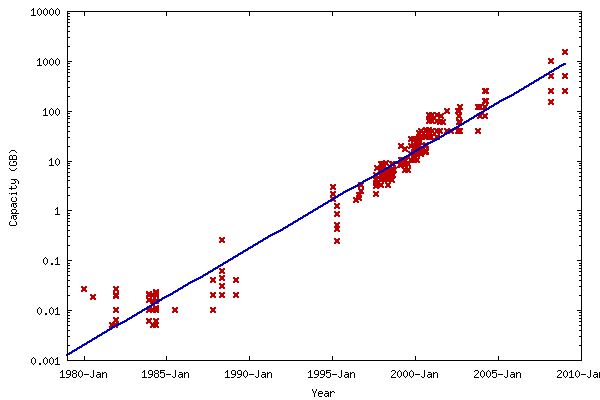
\includegraphics[scale=0.5]{HDDOverTime.png}
		\caption{Zmiana pojemności dysków w latach}
\end{figure}

Ponadto, przechowywane dane są różnych typow, z których wiele może mieć narzucone pewne wymagania
w predkości odczytu. Na przykład gdy otwieranie dużego pliku tekstowego zajmuje kilka, lub
kilkanaście minut, nie jest to tak uciążliwe jak kilkusekundowe wczytywanie każdej klatki
pliku multimedialnego.

Standardowe rozwiązania systemow przechowywania danych nie pozwalają na chwilę obecną
na zarządzanie dostępem do zasobów dysku indywidualnie dla każdego procesu operującego na plikach
(poza systemem operacyjnym \emph{Nemesis}\footnote{http://www.cl.cam.ac.uk/research/srg/netos/old-projects/nemesis/}, który nie jest jednak kontynuowany od 1999r).
W telekomunikacji istnieją juz takie mechanizmy, znajdujące sie na prawie kazdym routerze - 
\textbf{Quality of Service (QoS)}.

Quality of Service jest zbiorem charakterystyk staniowiacych podstawe do zaspokajania potrzeb
uzytkownika, ktore pozwalaja na
\begin{itemize}
\item kształtowanie i ograniczenie przepustowośći
\item zapewnienie sprawiedliwego dostępu do zasobów
\item nadawanie priorytetów poszczególnym pakietom
\item buforowanie nadmiarowych pakietów
\item unikanie przeciążen
\end{itemize}

\section{Cel badawczy}
Do tej pory QoS używany był prawie wyłącznie do kontrolowania pakietów przesyłanych przez sieć.
Jednak nie ma przeszkód aby zaimplementować ten mechanizm w systemach przechowywania danych, co
pozwoli na kontrolowanie procesów operujacych na plikach.

System taki byłby szczególnie przydatny w strumieniowaniu dużych plików multimedialnych.
Zapewnienie minimalnej prędkości dysku podczas odczytu tych plików (oraz ograniczenie maksymalnej
prędkości dla mniej ważnych procesów) może znacząco podnieść wydajność
takich usług.

\subsection{Cel praktyczny}
W tym celu zaimplementowany zostanie system plików o nazwie \textbf{QoSFS}\footnote{Quality of Service Filesystem}, który przy pomocy rozszerzonych atrybutów
(xattrs) pozwoli na ustalanie charakterystyk (minimalna i maksymalna dostępna predkość dysku)
Quality of Service dla każdego pliku/folderu indywidualnie. 

\begin{figure}[h!]
	\centering
	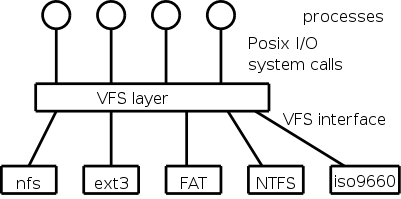
\includegraphics[scale=0.5]{vfs.png}
	\caption{Architektura Virtual File System}
\end{figure}

System będzie działał w oparciu o
\textbf{VFS (Virtual File System)} na systemie Linux.

Do wykonania QoSFS użyty zostanie moduł jądra, który umożliwia programowanie
logiki systemu plików - \tectbf{FUSE (Filesystem in USErspace)}. Jest to szeroko znany i uzywany
moduł, który stanowi bazę popularnego w GNU/Linux sterownika ntfs-3g\footnote{umożliwia
on dostęp odczytu/zapisu do systemu NTFS}.

\begin{figure}[h!]
	\centering
	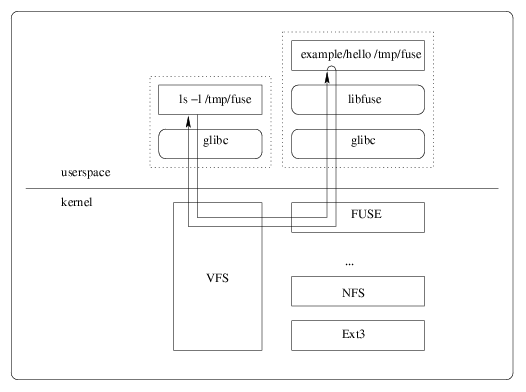
\includegraphics[scale=0.5]{fuse_structure.png}
		\caption{Struktura FUSE}
\end{figure}

FUSE pozwala na programowanie w przestrzeni użytkownika, oraz konfigurację poprzez
pliki i aktualizację wersji bez restartu.

\subsection{Cel teoretyczny}
Teoretyczną częścią pracy magisterskiej będzie analiza wykonanego systemu pod kątem przydatności,
opóźnień odczytu i zapisu oraz ewentualnych przeciążeń w komunikacji
oraz porownanie z rozwiązaniem zaproponowanym przez firme \emph{Red Hat} wystęepująacym
od wersji \emph{Red Hat Enterprise Linux OpenStack Platform 4}.

W tym celu zostaną napisane programy benchmarkowe wykonujace operacje
odczytu i zapisu na dużych plikach, które umożliwią analizę wykonanego rozwiązania.

\bibliographystyle{alpha}
\bibliography{mastersthesis}
\nocite{*}

\end{document}
